\section{Technique et gestion}
	\subsection{Suivi de l'avancement}
	\subsubsection{Backend}

\paragraph{Authentification} TODO Emile

\paragraph{HTTPS} Le service (lequel ?) est passé au HTTPS.

\paragraph{Réglages} La base de données des réglages est créée, ainsi que son API.

\paragraph{Droits d'accès à l'horaire} Échec fatal \rWalley

\paragraph{Base de données de l'horaire} TODO What do we have...
	
\subsubsection{Mobile}

\paragraph{Internationalisation} Offrir l'application en plusieurs langues s'avère beaucoup plus complexe que prévu étant donné le manque de synchronisme entre les composantes.

\paragraph{Incohérences UI} Des incohérences au niveau de l'UI ont été corrigées avec succès. 

\paragraph{Icône} L'application possède maintenant une icône unique et distinctive.

\paragraph{Notifications} Un registre des notifications existe désormais pour\dots %TODO Register

\paragraph{CAS} L'interface de CAS est désormais intégrée dans une webview.

\paragraph{Calendrier} La version 2 du calendrier est fonctionnelle.

\subsubsection{Gestion}

\paragraph{GitLab} La licence GitLab a pris fin, donc l'équipe est sous la version gratuite et limitée de la plateforme. La licence pour établissements d'enseignement tarde étant donné le trop grand nombre d'institutions intéressées.

\paragraph{JIRA} L'équipe rentre ses heures correctement dans JIRA, ce qui améliore l'allure des courbes.

\paragraph{Rapports} Toute l'équipe contribue aux rapports via GitLab sans avoir nécessairement besoin d'une distribution \LaTeX{} locale.




	\subsection{Écarts et révision de la planification}
	\begin{figure}[H]
		\centering
		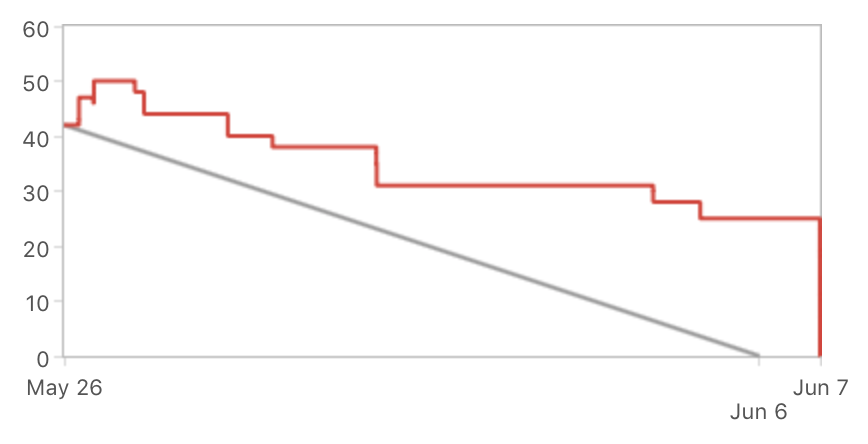
\includegraphics[width=0.65\textwidth]{Figures/burndownChart}
		\caption{Burndown Chart du sprint 1}
		\label{fig.burndowm}
	\end{figure}		

	\subsection{Prévisions pour la prochaine itération}
	\subsubsection{Backend}
% Auth Oauth2, être capable de faire un DIFF sur un JSON d'horaire, faire un API pour recevoir les API

\paragraph{Authentification} Posséder une méthode d'authentification avec OAuth2 fonctionnelle.

\paragraph{DIFF} Être en mesure d'effectuer nous-mêmes un DIFF sur un fichier JSON enregistré localement.

\paragraph{API} Concevoir un API pour recevoir les notifications de l'autre équipe.

\subsubsection{Mobile}
% Corriger éléments UI, faire itération 2 du calendrier custom, intégration avec backend, notifications

\paragraph{UI} Corriger certains éléments incohérents de l'UI (titres dédoublés, barres de navigation).

\paragraph{Calendrier} Produire la 2\ieme{} itération du calendrier qui se connectera au serveur.

\paragraph{Authentification} Commencer à intégrer l'authentification du \emph{backend} dans l'application mobile.

\paragraph{Notification} Développer des notifications de base sur l'application.

\paragraph{I18n} Développer l'internationalisation sur l'application pour se faire approuver sur l'App Store.

\subsubsection{Gestion}
% Peaufiner le pointage des tâches (temps), établir standards GIT

\paragraph{Pointage} Peaufiner le pointage des tâches en ce qui a trait au temps requis pour chacune.

\paragraph{Git} Établir des standards pour l'utilisation de Git.

	\subsection{Risques importants}
	\section{Problèmes rencontrés}
	\subsection{Backend}
	\paragraph{Horarius} L'accès au JSON d'horarius s'avère plus complexe que prévu. La version iCal n'est pas présentée de la même manière, même si convertie en JSON, ce qui nécessiterait davantage de manipulation de données.
	
	\subsection{Mobile}
	L'offre de frameworks de calendriers en React Native avoisine la nullité. Cependant, l'équipe ne veut pas faire la conception calendrier à partir de rien, car c'est un défi énorme. Il y a beaucoup de \emph{edge cases} à penser et il est très difficile de faire du beau UI sans un designer très expérimenté. Nous tenterons jusqu'au bout d'utiliser les \emph{plugins} qui existent et de les étendres avant de faire notre propre implémentation.
	
	\subsection{Gestion}
	L'équipe aura avantage à instaurer des normes à suivre sur Git. Se rapprochant de la fin du baccalauréat, chaque membre de l'équipe possède sa propre expérience en entreprise de l'outil et sa propre définition de \og bonnes pratiques \fg, ce qui mène parfois à de petits débats.